\begin{enumerate}
%
\item 
\begin{align}
\label{eq:5.2.3_alg_conic_a}
\brak{a} 12x^{2} - 7x + 1
\end{align}
can be expressed  as 
\begin{align}
\label{eq:5.2.3_vec_conic_a}
\vec{x}^T \myvec{12 & 0\\0 & 0}\vec{x}+ \myvec{-7 & 0}\vec{x}+1=0
\end{align}
To find roots using \ref{eq:5.2.3_vec_conic_a}, substitute
\begin{align}
y=0
\\
\implies 
12x^{2}-7x+1=0
\\
x=\frac{1}{3}, \frac{1}{4}
\end{align}
Hence $\brak{x-\frac{1}{3}}$ and $\brak{x-\frac{1}{4}}$ are the factors
\begin{align}
\implies \brak{3x-1}\brak{4x-1}=12x^{2} - 7x + 1 
\end{align}

The following code sketches the graph of \ref{eq:5.2.3_alg_conic_a} in figure \ref{fig:5.2.3_conic2a}
\begin{lstlisting}
solutions/3/codes/conic2/conic2a.py
\end{lstlisting}
\begin{figure}[!ht]
\centering
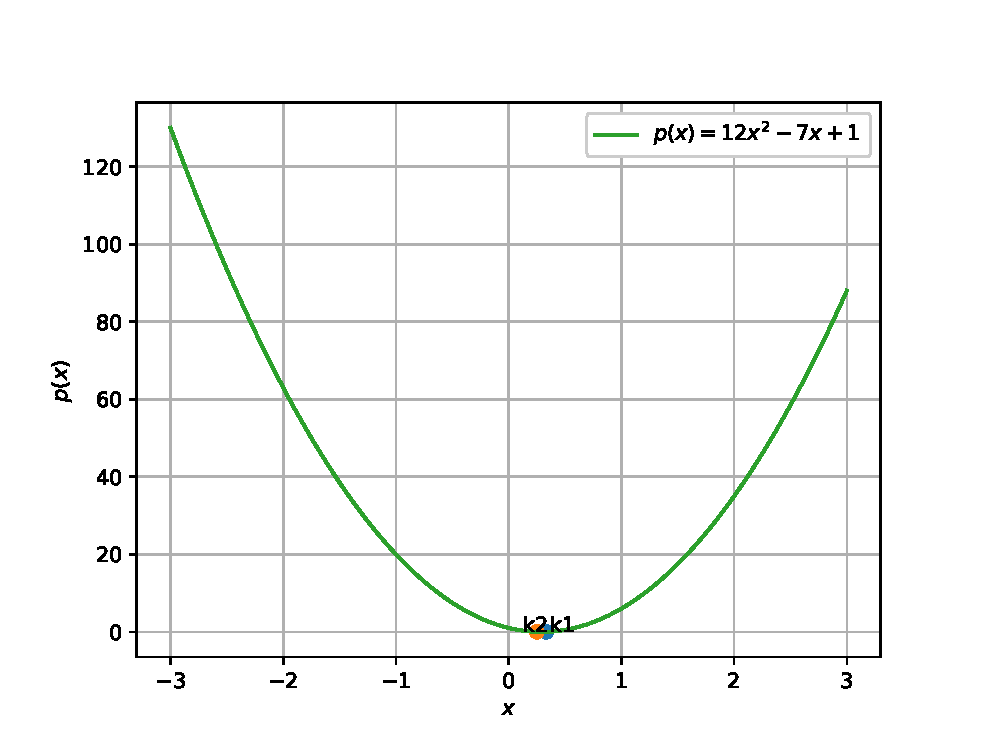
\includegraphics[width=\columnwidth]{./solutions/3/codes/conic2/pyfigs/conic2a.eps}
\caption{Graph of $12x^{2} - 7x + 1$}
\label{fig:5.2.3_conic2a}
\end{figure}


\item 
\begin{align}
\label{eq:5.2.3_alg_conic_b}
\brak{b} 6x^{2} + 5x -6
\end{align}
can be expressed  as 
\begin{align}
\label{eq:5.2.3_vec_conic_b}
\vec{x}^T \myvec{6 & 0\\0 & 0}\vec{x}+ \myvec{5 & 0}\vec{x} -6 =0
\end{align}
Substituting $y=0$ in equation \ref{eq:5.2.3_vec_conic_b} to find roots,
\begin{align}
\implies 
6x^{2}+5x-6=0
\\
x=\frac{-3}{2}, \frac{2}{3}
\\
\brak{2x+3}\brak{3x-2}= 6x^{2} + 5x -6
\end{align}
The following code sketches the graph of \ref{eq:5.2.3_alg_conic_b} in figure \ref{fig:5.2.3_conic2b}
\begin{lstlisting}
solutions/3/codes/conic2/conic2b.py
\end{lstlisting}
\begin{figure}[!ht]
\centering
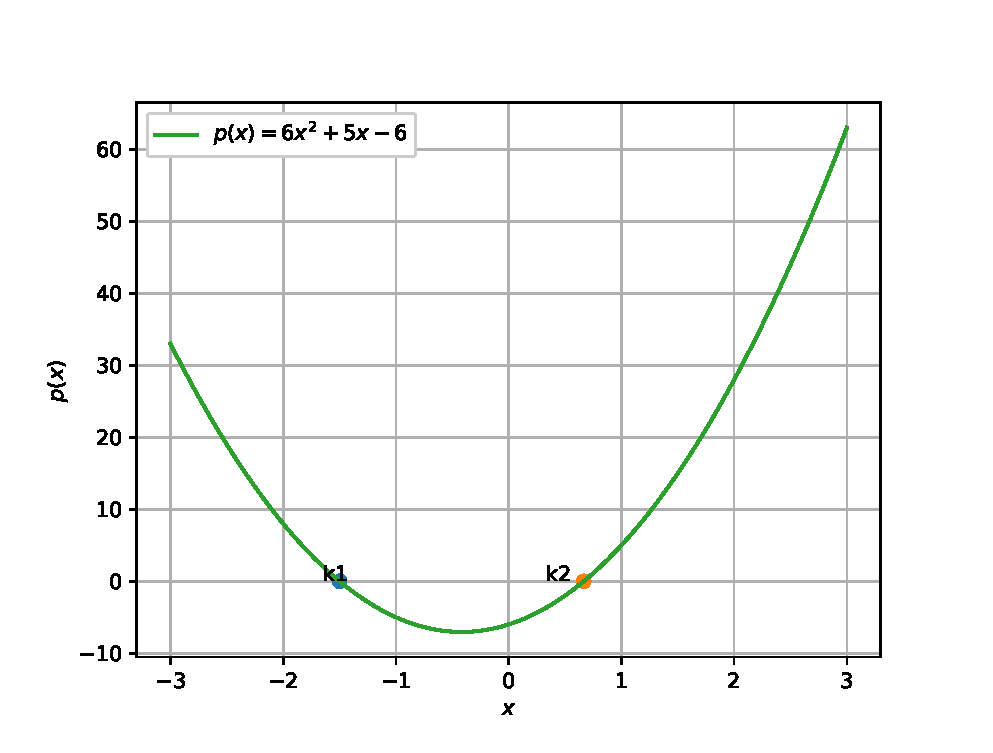
\includegraphics[width=\columnwidth]{./solutions/3/codes/conic2/pyfigs/conic2b.eps}
\caption{Graph of $6x^{2} + 5x -6$}
\label{fig:5.2.3_conic2b}
\end{figure}

\item 
\begin{align}
\label{eq:5.2.3_alg_conic_c}
\brak{c} 2x^{2} + 7x +3
\end{align}
can be expressed  as 
\begin{align}
\label{eq:5.2.3_vec_conic_c}
\vec{x}^T \myvec{2 & 0\\0 & 0}\vec{x}+ \myvec{7 & 0}\vec{x} +3 =0
\end{align}
Substituting $y=0$ in equation \ref{eq:5.2.3_vec_conic_c},
\begin{align}
\implies 
2x^{2}+7x+3=0
\\
x=\frac{-1}{2},-3
\\
\brak{2x+1}\brak{x+3}= 2x^{2} + 7x +3
\end{align}

The following code sketches the graph of \ref{eq:5.2.3_alg_conic_c} in figure \ref{fig:5.2.3_conic2c}
\begin{lstlisting}
solutions/3/codes/conic2/conic2c.py
\end{lstlisting}
\begin{figure}[!ht]
\centering
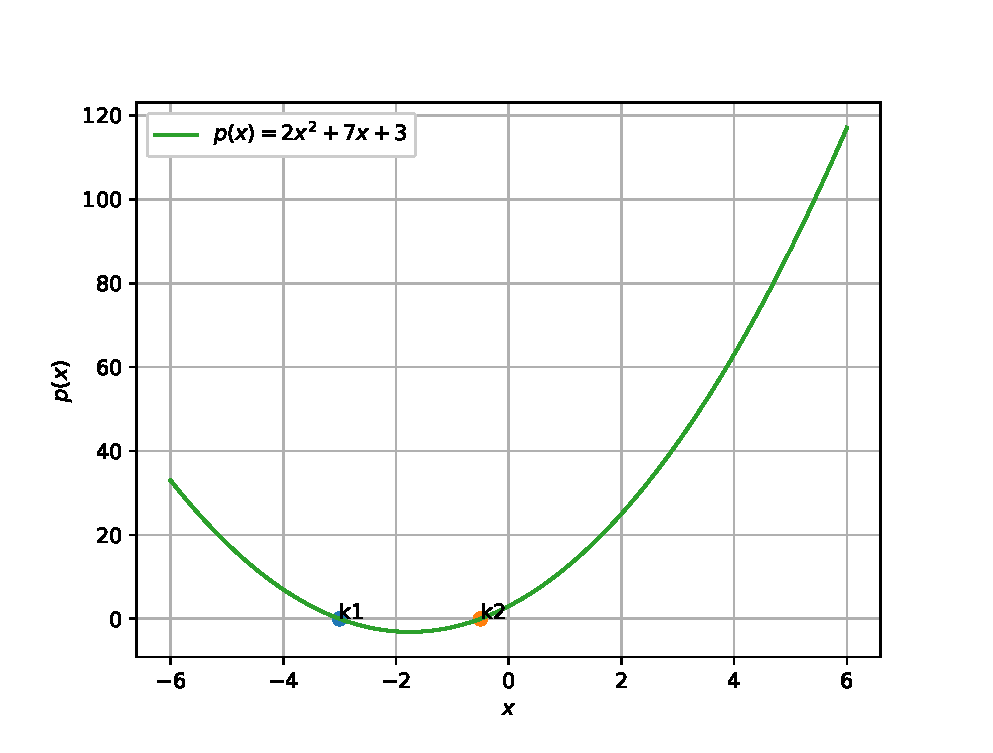
\includegraphics[width=\columnwidth]{./solutions/3/codes/conic2/pyfigs/conic2c.eps}
\caption{Graph of $2x^{2} + 7x +3$}
\label{fig:5.2.3_conic2c}
\end{figure}


\item 
\begin{align}
\label{eq:5.2.3_alg_conic_d}
\brak{d} 3x^{2} -x -4
\end{align}
can be expressed  as 
\begin{align}
\label{eq:5.2.3_vec_conic_d}
\vec{x}^T \myvec{3 & 0\\0 & 0}\vec{x}+ \myvec{-1 & 0}\vec{x} -4 =0
\end{align}
Substituting $y=0$ in equation \ref{eq:5.2.3_vec_conic_c},
\begin{align}
\implies 
3x^{2}-x-4=0
\\
x=\frac{4}{3},-1
\\
\brak{3x-4}\brak{x+1}= 3x^{2} -x -4
\end{align}

The following code sketches the graph of \ref{eq:5.2.3_alg_conic_d} in figure \ref{fig:5.2.3_conic2d}
\begin{lstlisting}
solutions/3/codes/conic2/conic2d.py
\end{lstlisting}
\begin{figure}[!ht]
\centering
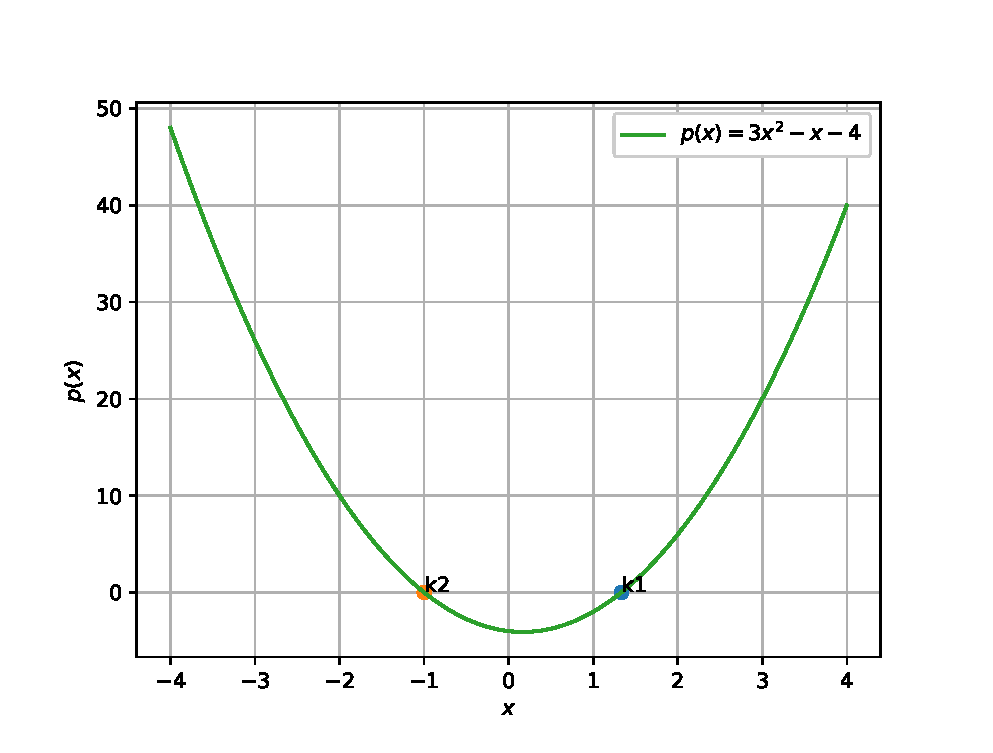
\includegraphics[width=\columnwidth]{./solutions/3/codes/conic2/pyfigs/conic2d.eps}
\caption{Graph of $3x^{2} -x -4$}
\label{fig:5.2.3_conic2d}
\end{figure}


\end{enumerate}
